\documentclass[crop,tikz]{standalone}
\usetikzlibrary{backgrounds}
\colorlet{blue}{cyan}
\tikzset{
  inverted/.style = {
    every path/.style = {draw=white,text=white},
    background rectangle/.style={fill},
    show background rectangle
  }
}

\tikzset{>=latex}
\usetikzlibrary{patterns}

\begin{document}
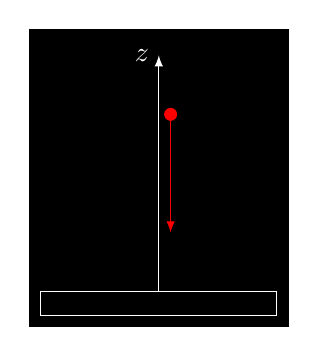
\begin{tikzpicture}[inverted,scale=1.5]
  \draw[->] (1,0) -- (1,2) node[left] {$z$};
  \coordinate (r) at (1.1,1.5);
  \draw[red,->] (r) -- ++(0,-1);
  \draw[red,fill] (r) circle (0.05);
  \draw (0,0) -- (2,0);
  \pattern[pattern=north east lines] (0,0)--(2,0)--(2,-0.2)--(0,-0.2)--cycle;
\end{tikzpicture}
\end{document}
